\chapter{经典函数公式}
论文中用到的经典函数公式如下。\\
\noindent{\bfseries (Sigmoid Function)}
Sigmoid 函数定义为
\[
\operatorname{Sigmoid}(x)=\frac{1}{1+e^{-x}}.
\]\\
\noindent{\bfseries (ReLU Function)}
ReLU 函数定义为
\[
\operatorname{ReLU}(x)=\max(0,x).
\]\\
\noindent{\bfseries (Leaky ReLU Function)}
Leaky ReLU 函数定义为
\[
\operatorname{LeakyReLU}(x)=\begin{cases}x,&x\geq0\\
\alpha x,&x<0\end{cases}
\]
其中 $\alpha$ 是一个较小的常数，通常取值为 0.01。\\

\chapter{用于定量比较的指标公式}
\label{cha:app_metrics}
章节~(\ref{sec:metrics}) 中提到的用于定量比较的指标公式如下。其中 $TP$、$TN$、$FP$ 和 $FN$ 分别表示真正例、真反例、假正例和假反例的数量。\\

\noindent{\bfseries (Precision)}
精确率定义为
\[
\text{Precision} = \frac{TP}{TP + FP}
\]
\noindent{\bfseries (Recall)}
召回率定义为
\[
\text{Recall} = \frac{TP}{TP + FN}
\]

\noindent{\bfseries (F1 Score)}
F1 分数定义为
\[
\text{F1 Score} = 2 \times \frac{\text{Precision} \times \text{Recall}}{\text{Precision} + \text{Recall}}
\]
\noindent{\bfseries (Matthews Correlation Coefficient)}
马修斯相关系数定义为
\[
\text{MCC} = \frac{TP \times TN - FP \times FN}{\sqrt{(TP + FP)(TP + FN)(TN + FP)(TN + FN)}}
\]
\noindent{\bfseries (Intersection over Union)}
交并比定义为
\[
\text{IoU} = \frac{TP}{TP + FP + FN}
\]
\noindent{\bfseries (Accuracy)}
准确率定义为
\[
\text{Accuracy} = \frac{TP + TN}{TP + TN + FP + FN}
\]

\chapter{\textrm{NECDNet} 额外检测结果}
\label{cha:app_necdnet_results}
\begin{figure}[!htbp]
    \centering
    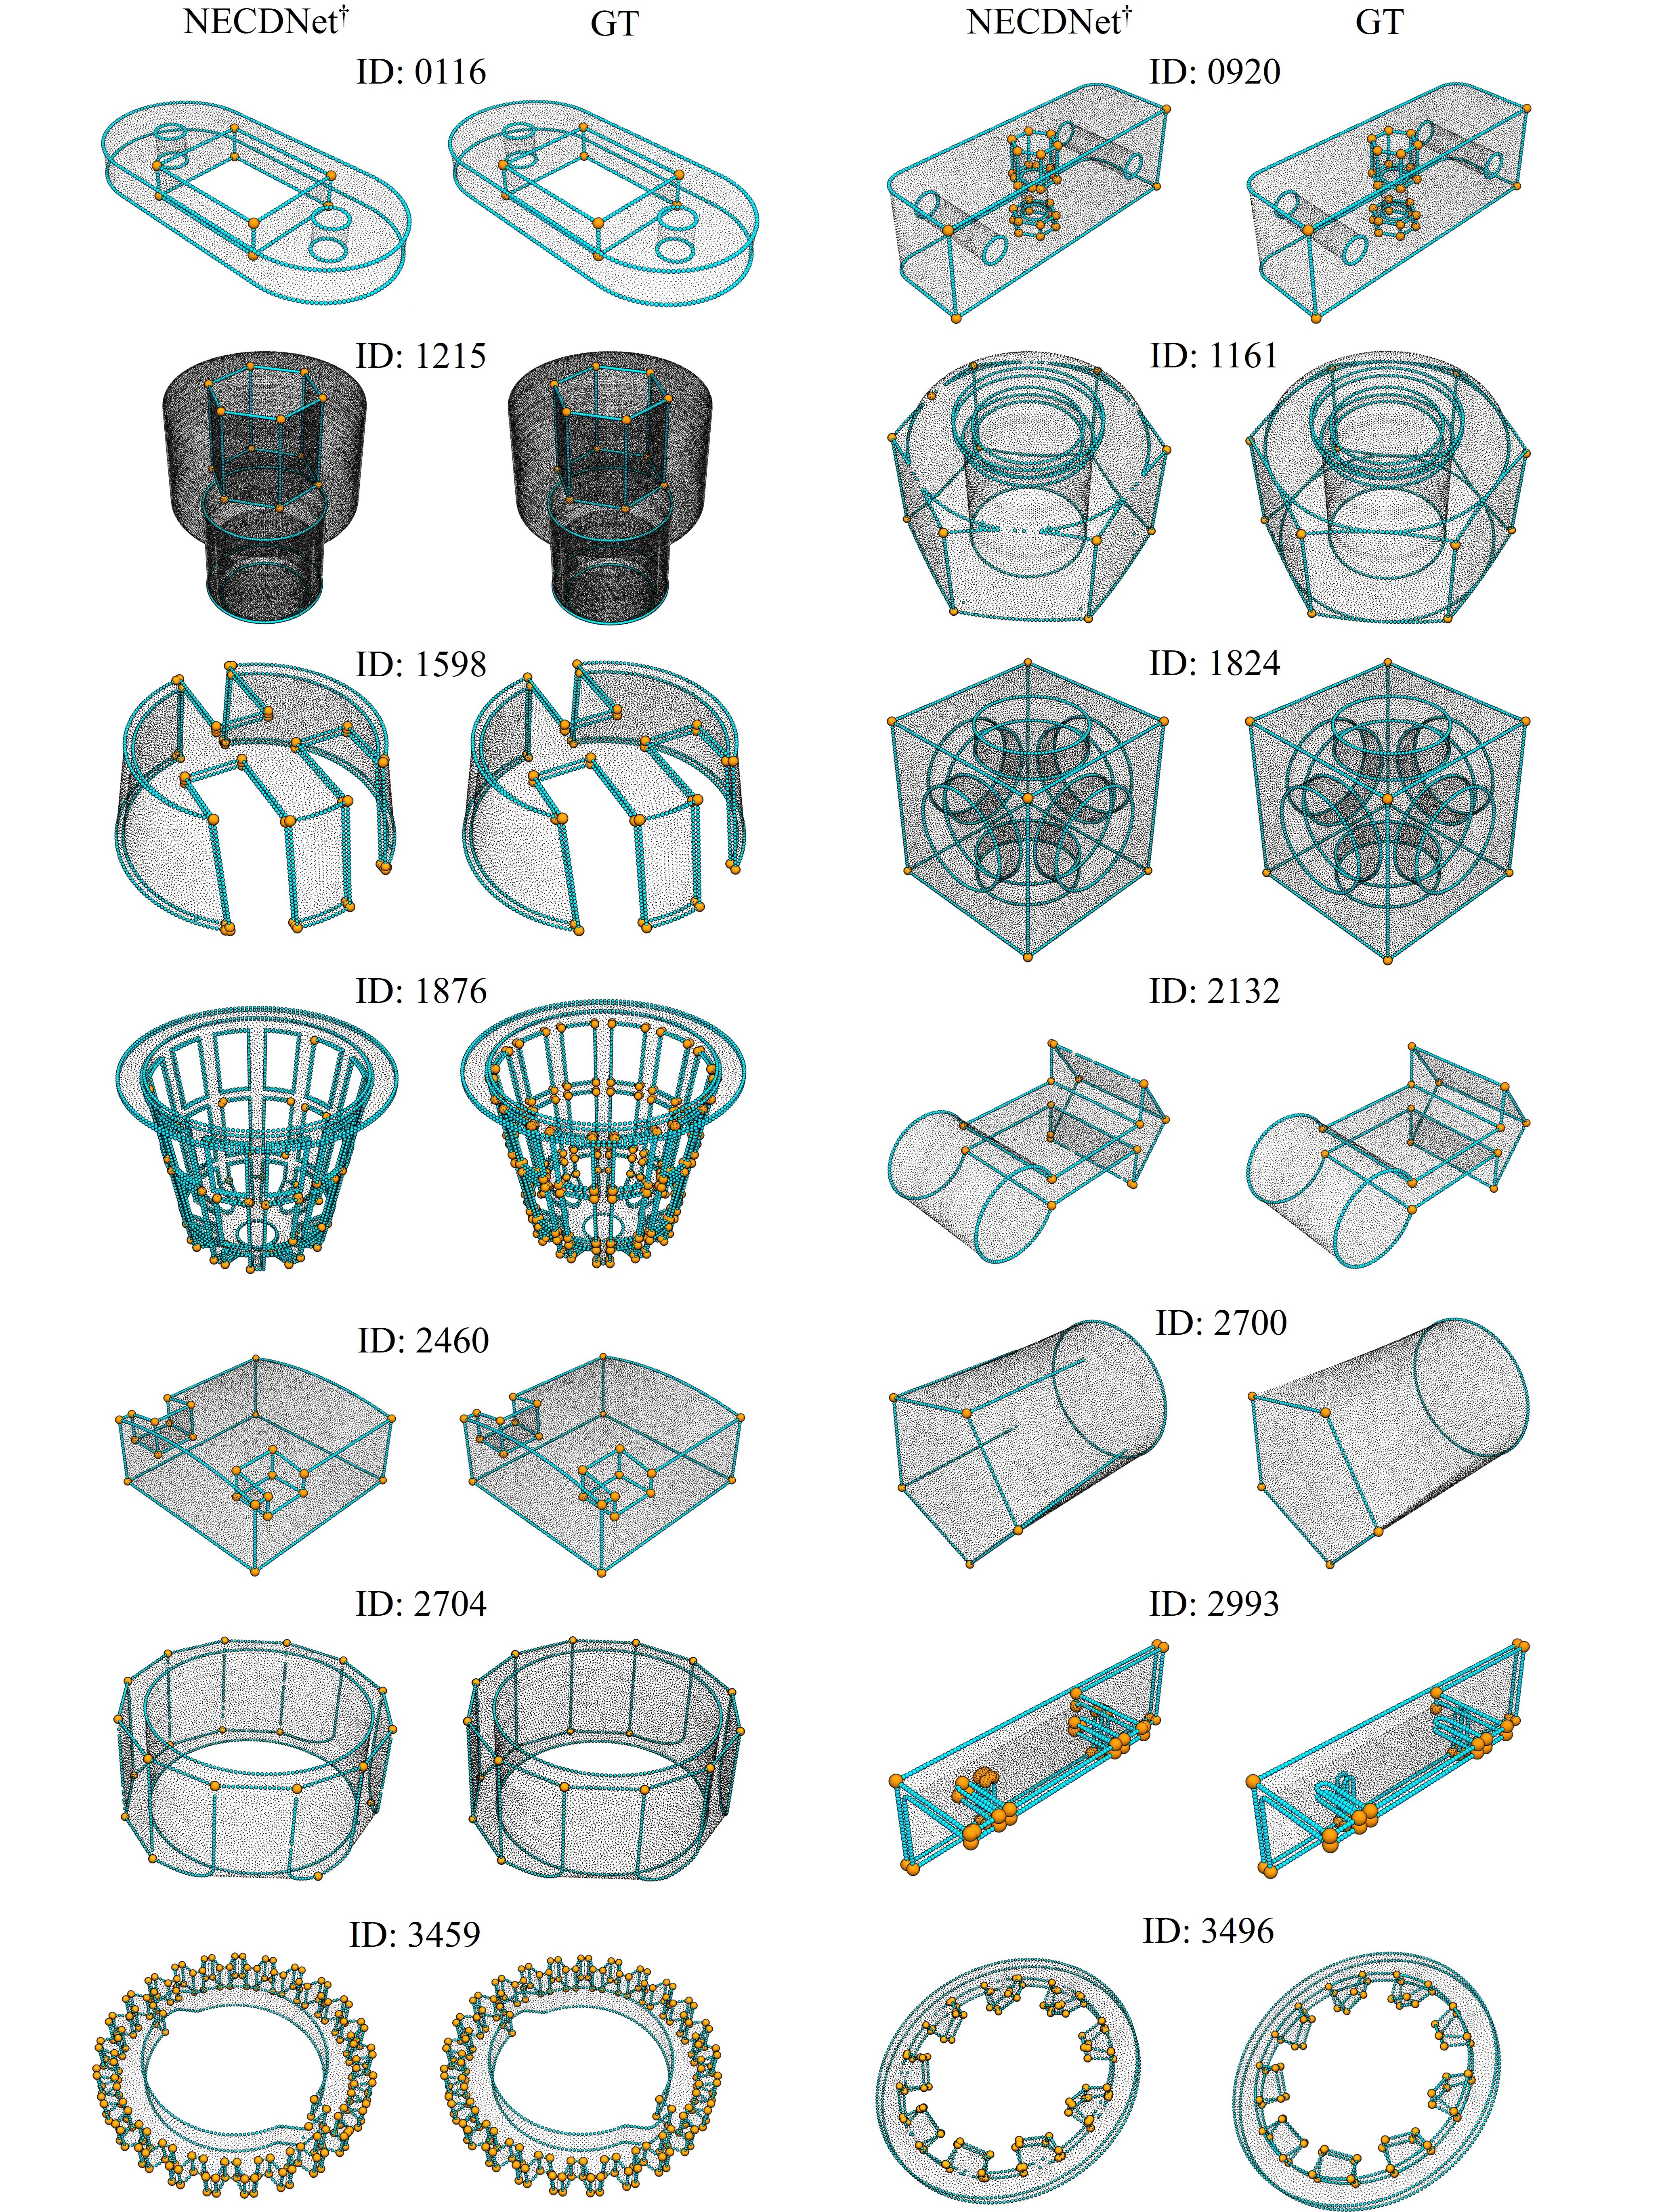
\includegraphics[width=0.95\textwidth]{NECDNet/additional_result.jpg}
    % \bicaption{NECDNet 在 ABC-Corner 数据集上的额外检测结果示例}{Additional detection results of NECDNet on the ABC-Corner dataset.}
    \label{fig:appendix_necdnet_results}
\end{figure}

\chapter{额外测试物体上的抓取构型分布图}

\begin{figure}[!htbp]
    \centering
    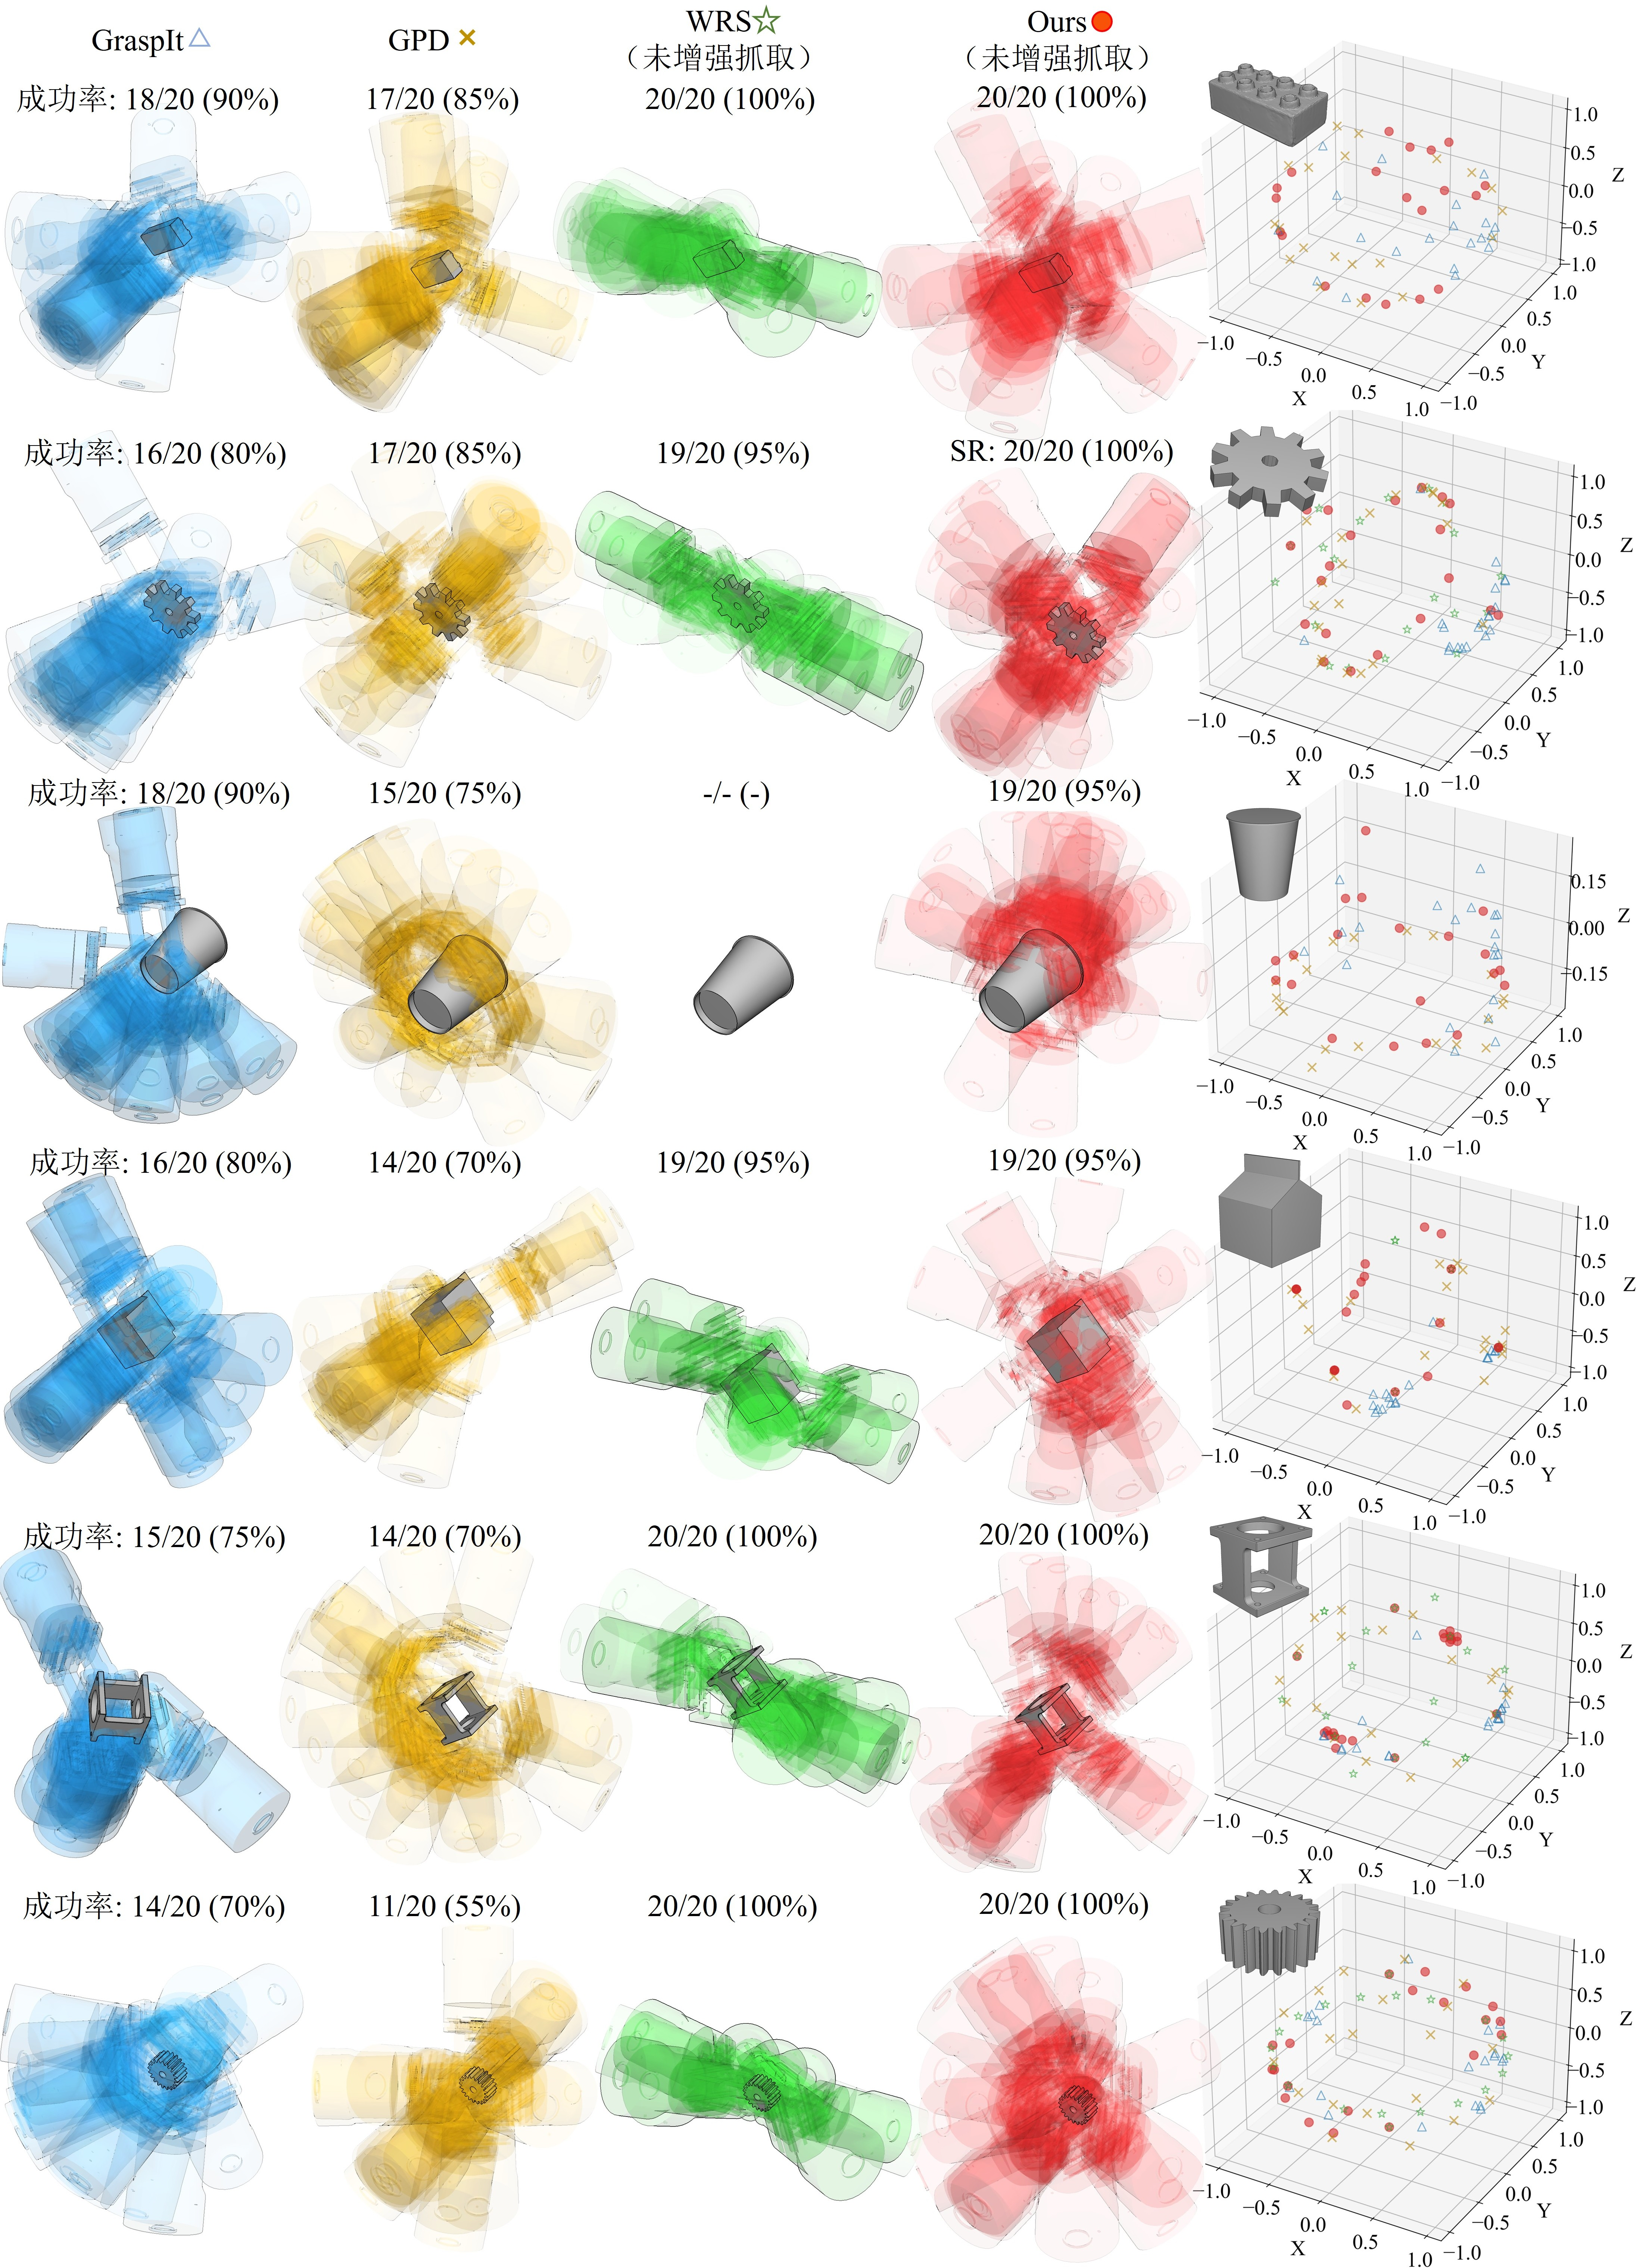
\includegraphics[width=0.95\textwidth]{FBGrasp/grasp_distribution.jpg}
    % \bicaption{在其余 7 种测试物体上的抓取构型分布图}{Grasp configuration distribution on the remaining 7 test objects.}
    \label{fig:appendix_grasp_distribution}
\end{figure}

